\chapter{Asking Orlando Millionaires How They Got Rich}

This chapter follows a School of Hard Knocks interview, curated by LazyingArt LLC. The material is not blackboard mathematics, but it does have a definite analytic spine: learning expenditures are treated as capital, price is separated from underlying value, a business is stabilized by multiple revenue verticals, wealth is described as an allocation problem rather than a raw income target, and credit is presented as a lever that can enlarge operational room. We keep the spoken order, because the sequence matters: first credibility, then decision rules, then structure, then compounding, and finally leverage.

\section{Cold Open and Sampling Frame}

The lecture begins not with an argument but with a promise. We are shown, in compressed form, a mentor paid \$55{,}000, a business scaled above \$5 million a year, yearly revenue claims in the eight-figure range, and a sharp question about how rich and poor people evaluate money. Only then does the host reset the scene in Orlando at Funnel Hacking Live and tell us what the episode will do: it will sample entrepreneurs and ask how they became millionaires, what mechanisms produced wealth in their industries, and how a viewer might begin the same path.

This is important for the way we read the chapter. The montage is not yet the proof; it is the statement of stakes. The subsequent interviews are the actual evidence, and each one is organized around a transfer principle rather than around biography alone.

\section{Value Before Price}

The first speaker earns the right to generalize by giving scale first: roughly fifteen years in business, roughly \$13 million in a single year, and a claim that about \$500{,}000 spent learning sales and marketing turned into \$33 million. Before we are asked to believe a doctrine, we are given a conversion from learning cost to business revenue.

\begin{equation}
m_{\text{learn}}
=
\frac{R_{\text{learn}}}{C_{\text{learn}}}
=
\frac{33{,}000{,}000}{500{,}000}
=
66.
\end{equation}

We should be careful: this is not audited profit, and it is not a universal law. It is a speaker's way of saying that education, masterminds, and market skill were not consumption; they were treated as productive capital.

\subsection{Question \& Answer}

\paragraph{Question.} What separates the wealthy from the middle class or poor in the way they think about money?

\paragraph{Answer.} The lecture answers with a staged little problem. A bag is offered for \$1{,}000. The quick answer is to judge the price. The wealthy answer, in the speaker's formulation, is to ask what is inside. The point is not the bag itself; the point is that pricing without investigating value is a systematic error.

\begin{equation}
P_{\text{bag}}=\$1{,}000,
\qquad
V_{\text{inside}}=\$100{,}000,
\qquad
U_{\text{bag}}=V_{\text{inside}}-P_{\text{bag}}=\$99{,}000.
\end{equation}

This is the clearest mathematical rule in the early part of the lecture. We do not begin by asking what something costs. We begin by asking what we get, and then we ask what is lost by refusing to inspect it. The speaker compresses the rule into a blunt slogan: rich people worry about what they get, not what it costs.

\section{Sales, Symbol, and Brand Discipline}

From there the host asks about sales, but the answer does not stay at the level of closing scripts. The speaker moves at once to brand structure. The most durable personal brands, he says, are like superheroes because they stand clearly for something and clearly against something. He recommends taking a known archetype, extracting what it stands for and against, and then modifying it into a coherent personal identity. His own emblematic example is ``Iron Dan,'' adapted from Iron Man.

We may formalize the rule without pretending that the lecture stated it as a theorem. Let \(\mathcal{F}\) denote the set of declared commitments, and \(\mathcal{G}\) the set of declared rejections. Then an utterance or action \(a\) is brand-consistent only if it aligns with that pair.

\begin{equation}
\chi_{\text{brand}}(a)=1
\iff
a \text{ aligns with }(\mathcal{F},\mathcal{G}).
\end{equation}

This is a useful editorial reduction of the speaker's line that everything one says and does must fall into alignment with what one stands for or against. The later, more aggressive remarks about ignorance and business seriousness are garbled in the transcript, but the central mechanism is clear: a brand is not mere logo or slogan; it is repeated coherence.

The host's recap after this interview is structurally important. He says, in effect, that the speaker used analogy to reveal how poor people think: they do not ask the right questions. That recap gives us permission to carry the bag rule forward as a general decision rule, not just as a memorable clip.

\section{Recession-Proof Business and the Structure of Wealth}

The Marcus interview pivots from persuasion to architecture. The visible prompt is a shirt reading ``recession proof,'' and the question becomes how one builds a business that survives shocks. The answer is not mystical. The answer is plurality: every business should make money three or four ways, and in practice at least four verticals are recommended.

\begin{equation}
n_{\text{verticals}}\ge 4.
\end{equation}

The named or implied verticals are the core product or service, a digital product, an in-person event, and a high-ticket mentorship or program. The arithmetic example is deliberately modest. One does not need millions from each vertical for the structure to matter.

\begin{equation}
R_{\text{high-ticket}}
=
P_{\text{high-ticket}}N
=
50{,}000\times 4
=
200{,}000.
\end{equation}

\begin{figure}
\centering
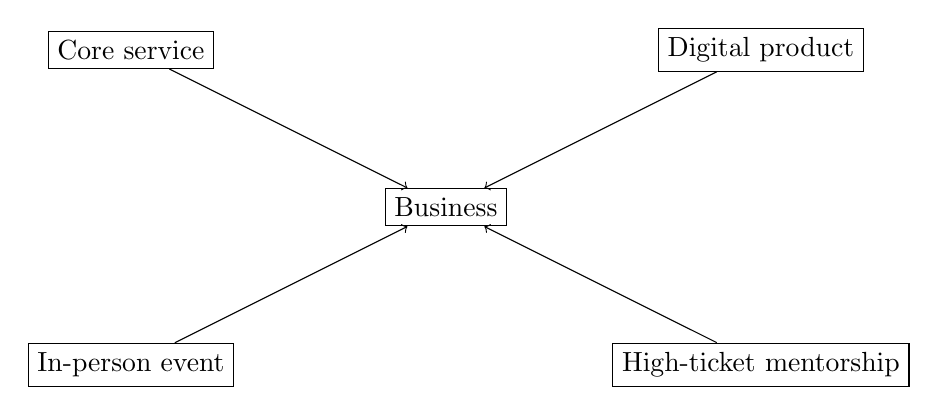
\begin{tikzpicture}
\node[draw, rectangle] (biz) at (0,0) {Business};
\node[draw, rectangle] (core) at (-4,2) {Core service};
\node[draw, rectangle] (digital) at (4,2) {Digital product};
\node[draw, rectangle] (event) at (-4,-2) {In-person event};
\node[draw, rectangle] (mentor) at (4,-2) {High-ticket mentorship};

\draw[->] (core) -- (biz);
\draw[->] (digital) -- (biz);
\draw[->] (event) -- (biz);
\draw[->] (mentor) -- (biz);
\end{tikzpicture}
\end{figure}

The lecture then makes a deeper move. Wealth, Marcus says, is not determined by a dollar amount but by structure. This is the moment at which the chapter leaves revenue boasting and becomes bookkeeping. A person earning \$100{,}000 can still build wealth if the money is divided properly across savings, equity growth, investment growth, and retained cash flow. In note form, the idea can be written as

\begin{align}
S &= sY, \qquad s\in[0.20,0.25], \\
\Delta W &\approx S+\Delta E_{\mathrm{RE}}+\Delta A_{\mathrm{inv}}+CF_{\mathrm{ret}}.
\end{align}

For the explicit income example used in the lecture, this gives

\begin{equation}
Y=\$100{,}000
\quad\Longrightarrow\quad
S\in[\$20{,}000,\$25{,}000].
\end{equation}

The point is not merely to save. The point is to convert income into positions that grow: real-estate equity, investment portfolio value, and retained business cash. Here the lecture's slogan is worth preserving: wealth is not what one makes; it is what one does with the money.

\section{Offense, Deployment, and the Poverty Trap}

The next interview sharpens the contrast. Money can be hoarded like acorns stuffed into a tree, or deployed like soldiers sent out to bring back more resources. The imagery is vivid, but the underlying distinction is analytic. The lecture contrasts defense, where one merely protects the current stock, with offense, where one uses present resources to expand future capacity.

This is not stated as a formal equation, but the operative principle is that capital should be assigned a growth task rather than a hiding place. In the speaker's rhetoric, each dollar is an active unit. That is why he criticizes the friends who stay in the same spot: their money is parked defensively, and so their decisions never compound.

\subsection{Question \& Answer}

\paragraph{Question.} If someone is stuck in a cycle of poverty, what are the first actionable steps?

\paragraph{Answer.} The answer is given by autobiography, and we should preserve that structure. At age \(21\), the speaker says, he left a sales job paying about \$150{,}000 for a job paying about \$30{,}000 because the second job promised learning. The lesson is not that lower wages are always better. The lesson is that early career years can be used to build human capital rather than merely to maximize immediate cash.

\begin{align}
Y_{\text{sales job}} &\approx \$150{,}000, \\
Y_{\text{learning job}} &\approx \$30{,}000.
\end{align}

We can write the compounding logic in the following minimal way. Let \(H_t\) denote human capital at age or time \(t\). Then

\begin{align}
H_{t+1} &= H_t+\Delta H_t, \\
Y_t &= f(H_t), \qquad f'(H_t)>0.
\end{align}

The lecture's claim is that the low-wage path may nonetheless dominate if it produces a much larger \(\Delta H_t\) over the formative period. The spoken reasoning is sequential and should remain sequential:

\begin{enumerate}
\item accept a short-run loss in wage income;
\item use the interval from roughly \(21\) to \(29\) to acquire knowledge, information, and saleable skill;
\item allow those skills to compound rather than remain static;
\item collect the higher earnings later, when the market now pays for accumulated competence rather than for raw effort alone.
\end{enumerate}

This is where the lecture is most explicit about timing. One should not compress it into a generic slogan about self-improvement. The actual mechanism is intertemporal: trade present consumption for future earning power.

\section{Credit, Mentorship, and Leverage Infrastructure}

The last interview turns from posture to operational leverage. The speaker begins with a critique of formal schooling: if one is taught by people earning \$40{,}000 to \$60{,}000 a year, one may acquire only the knowledge to reproduce that range. He then returns to the paid-mentorship theme from the opening montage and gives the largest single investment-to-scale comparison in the chapter.

\begin{equation}
m_{\text{mentor}}
=
\frac{R_{\text{post-mentor}}}{C_{\text{mentor}}}
\approx
\frac{5{,}000{,}000}{55{,}000}
\approx 90.9.
\end{equation}

Again, we record this as a gross revenue multiple, not as verified net return. The same caution applies to the later claim that the business is headed for eight figures; the transcript is garbled at one point, but the intended magnitude is clearly about \$10--11 million.

The credit mechanism is then stated as a chain. One adds tradelines, understood here as authorized-user history or comparable positive lines on a credit profile. This positively affects four of five credit metrics, raises a score from roughly \(600\) to \(700\), and thereby enlarges accessible credit to the range of \$50{,}000 to \$100{,}000. In schematic form, the claim is

\begin{equation}
T
\longrightarrow
\frac{4}{5}\text{ metrics improved}
\longrightarrow
C_{\text{score}}:600\to700
\longrightarrow
L_{\text{access}}\in[\$50{,}000,\$100{,}000].
\end{equation}

We should not embellish this into a full theory of credit scoring. The lecture does not enumerate the five metrics, and the software description itself is ambiguous in the transcript. But the practical logic is plain enough: better credit expands the balance sheet, and an expanded balance sheet can finance the start, growth, or scaling of a business.

What makes this closing section fit with the rest of the chapter is that it returns us to a theme already established in several forms. Paid mentorship leverages knowledge. Multiple verticals leverage one business into many cash streams. Human-capital compounding leverages time. Tradelines and score improvement leverage a credit profile into usable financial room. The lecture is not offering one master formula; it is offering a sequence of leverage devices.

\section{Summary}

The chapter begins with large numbers because the lecture wants authority before abstraction. But once the claims are in place, the underlying machinery is surprisingly consistent. First, we learn to distinguish value from price, so that opportunity is judged by upside rather than by sticker shock. Next, we see that sales at scale are linked to brand coherence: repeated alignment between what one stands for and what one does. Then the argument widens into business architecture and personal balance-sheet structure: many verticals, multiple growth channels, and disciplined allocation. After that, the lecture turns to dynamic posture, insisting that capital and time must be deployed offensively rather than hidden defensively. Finally, it arrives at explicit leverage infrastructure: mentorship, credit, tradelines, and access to capital.

These are not blackboard formulas, but they are formulas in another sense. They are update rules for commercial life. We move from a present stock of money, time, or reputation to a larger future state by choosing the right transformation. The lecture keeps repeating the same lesson in different costumes: do not merely hold; convert. Use money to build skill, use skill to build revenue, use revenue to build structure, and use structure to widen the set of future moves.